\documentclass[12pt,a4paper]{article}%
\usepackage[]{graphicx}\usepackage[]{color}
%% maxwidth is the original width if it is less than linewidth
%% otherwise use linewidth (to make sure the graphics do not exceed the margin)

%2multibyte Version: 5.50.0.2960 CodePage: 1252
\usepackage{amsfonts}
\usepackage{amssymb}
\usepackage[centertags]{amsmath}
\usepackage{graphicx}%
\usepackage{natbib}
\usepackage{color}
\usepackage[dvipsnames,svgnames*]{xcolor}
\usepackage{array}
\usepackage[hidelinks]{hyperref}
\usepackage[font=small,skip=5pt]{caption}
\usepackage[aboveskip=2pt]{subcaption}
\usepackage{amsmath}
\usepackage{amsthm}
%\usepackage{tikz}
%\usetikzlibrary{bayesnet}
\usepackage{url}
\usepackage{ulem}
\usepackage{afterpage}
\setcounter{MaxMatrixCols}{30}
\providecommand{\U}[1]{\protect\rule{.1in}{.1in}}
\newtheorem{theorem}{Theorem}
\newtheorem{acknowledgement}[theorem]{Acknowledgement}
\newtheorem{axiom}[theorem]{Axiom}
\newtheorem{case}[theorem]{Case}
\newtheorem{claim}[theorem]{Claim}
\newtheorem{conclusion}[theorem]{Conclusion}
\newtheorem{condition}[theorem]{Condition}
\newtheorem{conjecture}[theorem]{Conjecture}
\newtheorem{corollary}[theorem]{Corollary}
\newtheorem{criterion}[theorem]{Criterion}
\newtheorem{definition}[theorem]{Definition}
\newtheorem{example}[theorem]{Example}
\newtheorem{exercise}[theorem]{Exercise}
\newtheorem{lemma}[theorem]{Lemma}
\newtheorem{notation}[theorem]{Notation}
\newtheorem{problem}[theorem]{Problem}
\newtheorem{proposition}[theorem]{Proposition}
\newtheorem{remark}[theorem]{Remark}
\newtheorem{solution}[theorem]{Solution}
\newtheorem{summary}[theorem]{Summary}
\setlength{\topmargin}{0in}
\setlength{\oddsidemargin}{0.1in}
\setlength{\evensidemargin}{0.1in}
\setlength{\textwidth}{6.5in}
\setlength{\textheight}{8.25in}
\numberwithin{equation}{section}
\setlength\parindent{0pt}
\begin{document}

Model:
\begin{align*}
y_t &= \exp(x_t/2) z_t \\
x_t &= \mu + \phi (x_{t-1} - \mu) + \sigma u_t
\end{align*}
with $u_t, z_t \overset{iid}{\sim} N(0, 1)$ for all $t$.

Priors:
\begin{align*}
\mu &\sim N(0, 10) \\
\tau &= 0.5 (\phi + 1) \sim B(20, 1.5) \\
\sigma^2 &\sim IG(2.5, 0.025) \\
X_0 &\sim N\left(\mu, \frac{\sigma^2}{1 - \phi^2}\right)
\end{align*}

DGP Values:
\begin{align*}
\mu &= -0.5 \\
\phi &= 0.8 \\
\sigma^2 &= 0.02 \\
T &= 500
\end{align*}

Methods:
\begin{itemize}
\item PMMH (Andrieu, Doucet and Holenstein 2010): 20,000 draws, first 10,000 discarded. $\theta^{(i)} \sim MVN(\theta^{(i-1)}, 0.05)$ proposal distribution. Sample $\{\mu, \phi, \sigma^2, x_{0:T} \}$ jointly, then use all draws to estimate $\hat{p}(x_{T+1}) \approx \sum_{i=1}^10000 p(x_{T+1} | x_T^{(i)}, \mu^{(i)}, \phi^{(i)}, \sigma^{2,(i)}) / 10000$.
\item VB: Multivariate normal approximation of $\left\{\mu, \phi, \ln \left(\sigma^2\right), x_{T+1} \right\}$ using 
\begin{align*}
\ln(p(\mu, \phi, \sigma^2, x_{T+1}, y_{1:T})) &\approx \ln\left(p\left(\mu, \phi, \sigma^2\right)\right) + \ln \left(\hat{p}\left(y_{1:T} |\mu, \phi, \sigma^2\right)\right) \\
&+ \ln \left(\sum_{k=1}^N \pi_T^{(k)} p\left(x_{T+1} | \mu, \phi, \sigma^2, x_T^{(k)}\right)\right),
\end{align*}
where $\hat{p}$ denotes a particle filter estimate and $\{x_T^{(k)}, \pi_T^{(k)} \}$ denote a point mass and associated weight of the particle estimate of $\hat{p}(x_T | \mu, \phi, \sigma^2, y_{1:T})$ for particle $k = 1, 2, \dots, N$.
\end{itemize}

\newpage

Results: Posterior Mean and Standard Deviation for PMMH and VB fit to twenty different datasets.

\begin{figure}[h]
\centering
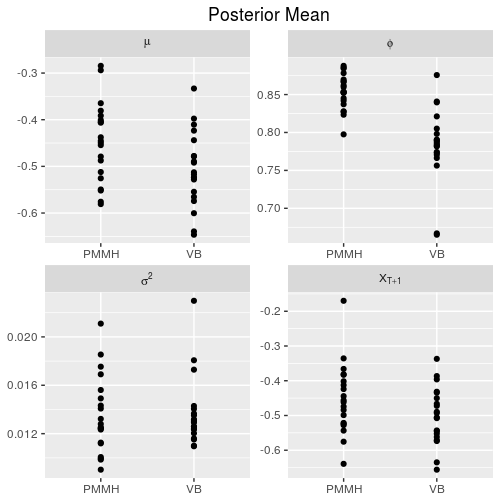
\includegraphics[width=0.45\textwidth]{mean}
\end{figure}

\begin{figure}[h]
\centering
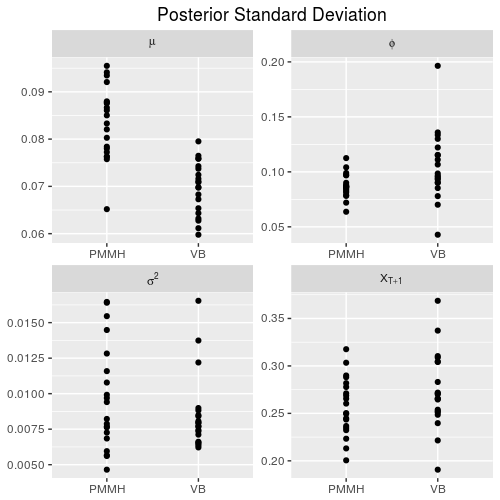
\includegraphics[width=0.45\textwidth]{standardDev}
\end{figure}


\end{document}